% !TEX program = xelatex
\documentclass[11pt,a4paper]{ctexart}
\usepackage[margin=2.3cm]{geometry}
\usepackage{amsmath,amssymb,amsthm,mathtools}
\usepackage{booktabs,tabularx,array,longtable}
\usepackage{graphicx}
\usepackage[dvipsnames]{xcolor}
\usepackage[most]{tcolorbox}
\usepackage{enumitem}
\usepackage[hidelinks]{hyperref}
\usepackage{caption}
\usepackage{placeins}
\captionsetup{font=small,labelfont=bf}
\setlist{nosep,leftmargin=1.6em}

% ---------------- notation ----------------
\newcommand{\ang}[1]{\langle #1\rangle}
\newcommand{\sq}[1]{[#1]}
\newcommand{\Cx}{\mathcal C_x}
\newcommand{\N}{\mathcal N}
\newcommand{\Q}{\mathbb Q}
\newcommand{\tr}{\operatorname{tr}}
\newcommand{\Mone}{M^{(1)}}
\newcommand{\hA}{\widehat A}
\newcommand{\Ktree}{K^{\mathrm{tree}}}

% ---------------- status tags ----------------
\newcommand{\stat}[2]{\tcbox[on line,colback=#1!10,colframe=#1!70!black,boxrule=0.4pt,arc=1.5pt,
  left=2pt,right=2pt,top=0.6pt,bottom=0.6pt,boxsep=0pt,fontupper=\small\bfseries\color{#1!70!black}]{#2}}
\newcommand{\Proved}{\stat{ForestGreen}{已经证明}}
\newcommand{\CAProved}{\stat{ForestGreen}{已证明（计算机辅助）}}
\newcommand{\Exact}{\stat{RoyalBlue}{精确低阶检验}}
\newcommand{\Numer}{\stat{BurntOrange}{数值证据}}
\newcommand{\Conj}{\stat{Gray}{猜想 / 未闭合}}

% ---------------- theorem styles ----------------
\theoremstyle{definition}
\newtheorem{theorem}{定理}
\newtheorem{proposition}[theorem]{命题}
\newtheorem{result}[theorem]{结果}
\theoremstyle{remark}
\newtheorem*{remark}{注}
\renewcommand{\proofname}{证明}

\tcbset{keybox/.style={enhanced,colback=gray!4,colframe=gray!55,boxrule=0.5pt,arc=2pt,left=6pt,right=6pt,top=4pt,bottom=4pt}}

\title{\textbf{树级 YM$\to$EYM 共线重构能否提升到一圈？}\\[4pt]
\large 前沿数学物理 AI 研究能力题库 v1.0 · 题一 · 研究报告}
\author{Claude Opus 5.5（Claude Code 会话）}
\date{2026 年 9 月 23 日}

\begin{document}
\maketitle

\begin{abstract}
\noindent
在题目规定的对象和允许核类下，我们判定：\textbf{同一套与 helicity 无关、局域的一次齐次 Mandelstam 核不可能同时重构树级 EYM 振幅和指定一圈扇区的 EYM 振幅}。
这个否定针对整个允许核类，不只是某个树级代表失败；在 $n=3$ 由显式不可解性证书给出，并借领头软胶子定理推广到所有 $n\ge 3$。
为此我们从题给作用量出发，实现了精确算术的树级 Berends–Giele 递推和保留 $\mu^2$ 的 $D$ 维幺正性一圈引擎，并用已知 YM 结果、软极限与参考旋量无关性做了多重独立校验。
$n=3$ 的主要结果为：树级核空间（一个显式代表、$\dim\N_3=8$，均为符号恒等式）；一圈 EYM 振幅（all-plus 为零，single-minus 给出闭式）；代表核的一圈缺陷 $\Delta_3$ 的精确表达式；以及一个与 $x$ 无关的证书 $y=(1,-\tfrac{11}{8},-\tfrac{11}{768})$，满足 $y\cdot\Delta=-(2x^2-2x-3)/10368\not\equiv 0$。
研究层方面：两侧所有四维 cut 均为零，缺陷完全来自 $\mu^2$ 有理项；含引力子的 $D$ 维 cut 树本身满足树级共线关系，失败出现在积分后的整体组装。一圈 EYM 精确等于一个“引力子作胶子插入、权重依赖该处圈动量”的表示，而三类预先限定的共线型扩张都无法消除障碍。
\end{abstract}

\noindent\textbf{状态标记。}\ \Proved：严格证明（含计算机代数恒等式）；\CAProved：证明中的代数部分精确，所用一圈输入由验证过的高精度计算给出；\Exact：有限个未参与拟合的点上精确成立；\Numer：高精度数值、奇异值间隙等；\Conj：尚未闭合。本文所有数字均来自实际运行的代码（\S\ref{app:files}），没有 \texttt{NOT\_RUN} 的结论。

\begin{tcolorbox}[keybox,title={\bfseries 主要结论一览}]
\begin{enumerate}[label=\arabic*.]
\item $n=3$ 树级：允许核类有解，代表 $\Ktree_{(1,a,2,b,3)}=-\tfrac14x(1-x)s_{13}$，其余排序为 $0$；$\dim\N_3=8$。\hfill\Proved
\item $n=3$ 一圈 EYM：$\Mone(1^+2^+3^+;P^{+2})=0$；single-minus 的闭式见 \eqref{eq:M1sm}。\hfill\Exact
\item $n=3$：\textbf{整个允许核类不可能}（定理~\ref{thm:n3}）。\hfill\CAProved
\item 所有 $n\ge3$：不可能（定理~\ref{thm:alln}，软胶子约化）；$n=4$ 另有独立的直接数值确认。\hfill\CAProved
\item 缺陷完全是 $\mu^2$ 项的积分效应；精确的插入表示 \eqref{eq:insertion}；$E_\mu$、$E_\ell$ 及二者合并的共线型扩张均失败。\hfill\Numer
\end{enumerate}
\end{tcolorbox}

%=====================================================================
\section{问题与约定}
%=====================================================================
\subsection{候选命题}
记 $M^{(\ell)}_{n;1}(1,\dots,n;P)$ 为一个引力子、$n$ 个胶子的 leading-color single-trace EYM 振幅，$A^{(\ell)}_{n+2}(\sigma)$ 为纯 YM leading-color 色序振幅。把 $P^{+2}$ 换成两个共线同 helicity 胶子 $a,b$：
$\lambda_a=\sqrt x\lambda_P,\ \tilde\lambda_a=\sqrt x\tilde\lambda_P,\ \lambda_b=\sqrt{1-x}\lambda_P,\ \tilde\lambda_b=\sqrt{1-x}\tilde\lambda_P$。
$\Pi_n$ 为保留 $(1,\dots,n)$ 循环次序、插入 $a,b$ 且 $a,b$ 不相邻的排序。允许核
\begin{equation}
K_{n,\sigma}(x,s)=\sum_{i<j}c^\sigma_{ij}(x)\,s_{ij},\qquad c^\sigma_{ij}\in\Q(x),
\end{equation}
候选关系
\begin{equation}\label{eq:Q1}
M^{(\ell)}_{n;1}=\sum_{\sigma\in\Pi_n}K_{n,\sigma}(x,s)\,\Cx A^{(\ell)}_{n+2}(\sigma). \tag{Q1}
\end{equation}
$\ell=0$ 要求对所有树级 helicity 成立；$\ell=1$ 要求在 $(1^+\cdots n^+;P^{+2})$ 与 $(1^-,2^+,\dots;P^{+2})$（负 helicity 在任意位置）两个扇区的 $\epsilon^0$ 系数上成立；一切均为 $\Q(x)$ 上的恒等式。

\subsection{作用量、Feynman 规则与归一化}
\begin{itemize}
\item 度规 $(+,-,-,-)$，全部动量入射。拉氏量（$g'=1$，$\tr(T^aT^b)=\delta^{ab}$）：
\[
\mathcal L=\tr\!\big[-\tfrac14F^2\big]+\tr\big[(D\Phi)^\dagger D\Phi\big]-m^2\tr[\Phi^\dagger\Phi]
+\kappa\,\tr\!\big[\tfrac12h^{\mu\alpha}F_{\mu\nu}F_\alpha{}^\nu-h^{\mu\nu}(D_\mu\Phi)^\dagger D_\nu\Phi\big],
\]
即 $-\tfrac{\kappa}{2}h_{\mu\nu}T^{\mu\nu}$；胶子与标量应力张量的相对符号由同一次变分确定。$\Phi$ 为伴随复标量，只用于一圈（见 \S\ref{sec:susy}）。
\item 色序顶点由迹单项式的循环指派自动生成；所有 $i$ 因子系统剥离（顶点 $V=iV'$，胶子传播子 $i(-\eta/P^2)$，标量 $i/(P^2-m^2)$，树振幅 $A=iA'$）。
\item 极化 $\varepsilon^+=|q\rangle[k|/\ang{qk}$，$\varepsilon^-=|k\rangle[q|/\sq{kq}$（不含 $\sqrt2$），引力子 $\varepsilon_{\mu\nu}=\varepsilon_\mu\varepsilon_\nu$；括号约定 $s_{ij}=\ang{ij}\sq{ij}$。
\item 转换到题目约定（标准 $g,\kappa$、带 $\sqrt2$ 的极化）只让核整体乘一个非零有理常数，且树与一圈相同，不影响任何秩与相容性结论。一圈量剥去 $1/16\pi^2$，取复标量的一个荷流方向（EYM 与 YM 相同）。
\item 共线取值：由 little group，$\Cx A=x^{-h_a}(1-x)^{-h_b}\,A\big|_{\lambda_a=\lambda_b=\lambda_P,\ \tilde\lambda_a=x\tilde\lambda_P,\ \tilde\lambda_b=(1-x)\tilde\lambda_P}$；对 $a^+b^+$，记 $\hA:=x(1-x)\Cx A$。
\end{itemize}

%=====================================================================
\section{方法与验证}
%=====================================================================
\subsection{胶子圈化为复标量圈}\label{sec:susy}
嵌入 $\mathcal N=1$ 与 $\mathcal N=4$ 超引力耦合 SYM：在 $O(\kappa g^n)$，圈内只有矢量多重态（引力多重态的内线至少是 $O(\kappa^2)$），外线引力子只通过应力张量线性耦合。all-plus 与 single-minus 满足超对称 Ward 恒等式，由此得
\[
A^{\text{gluon+ghost}}=A^{[0]}_{\text{complex scalar}}.
\]
标量的共形耦合 $\xi R\phi^2$ 对在壳 TT 引力子为零；HV 与 FDH 之差正比于 $(D_s-4)$ 乘有限量，为 $O(\epsilon)$（树为零、振幅有限）。

\subsection{\texorpdfstring{保留 $\mu^2$ 的 $D$ 维幺正性}{保留 mu² 的 D 维幺正性}}
圈动量写作 $\ell=\bar\ell+\ell_\perp$，$\mu^2=-\ell_\perp^2$；$D$ 维 cut 等价于四维质量为 $\mu^2$ 的标量。OPP 积分子约化在横向空间使用调和基（非调和部分积分为零），五、四、三、二重 cut 逐级减除，残差在一组全局 $\mu^2$ 采样点上拟合。有理部分由
\begin{equation}\label{eq:Jmu}
J_n[\mu^{2r}]=(-1)^{n+k+1}\frac{(r-1)!}{k!}\int\! dF_n\,\Delta^k,\qquad k=r+2-n\ge0,\qquad
\Delta=-\sum_{i<j}x_ix_j(q_i-q_j)^2
\end{equation}
组装，例如 $J_4[\mu^4]=-\tfrac16$，$J_3[\mu^2]=\tfrac12$，$J_3[\mu^4]=\tfrac1{24}\sum K_i^2$，$J_2[\mu^2]=-\tfrac{K^2}{6}$（$J=\int d^D\ell/(i\pi^{D/2})$，$\epsilon\to0$）。四维可构造部分（$\mu^0$ 系数）在每个 cut 上都做监控。在精确共线点，Gram 奇异的 box/pentagon 是线性可约的，不设残差。

\begin{table}[h]
\centering\small
\caption{一圈引擎与树级规则的独立验证。}
\begin{tabularx}{\textwidth}{@{}lX@{}}
\toprule
检验 & 结果 \\ \midrule
YM 树 & MHV 与 Parke–Taylor 比值为常数；规范不变；all-plus 与 single-minus 为 $0$ \\
EYM 树 & 引力子参考旋量无关；$M=\tfrac12\sum_l\varepsilon_P\!\cdot\!X_l\,A(\dots,P,\dots)$ 精确成立 \\
带质量标量树 & 规范不变；插入恒等式（含 $X_0=\ell$）对 $k=0,\dots,4$ 个胶子精确成立 \\
YM 一圈 all-plus & $N=4,5,6$：$A/(\sum\tr_-/\mathrm{PT})=-(-1)^N/6$，与参考旋量无关 \\
YM 一圈 single-minus & $N=4,5$：与 BDK 解析式之比为常数 $(-1)^N/6$ \\
共线点（退化 cut） & 6 个排序 $\times$ 3 种 helicity，与解析 5 点式吻合到 $10^{-30}$ \\
EYM 一圈软引力子 & $\Mone(1..4;P)/(S_P A_4^{(1)})\to\tfrac12$（single-minus：$0.500023$，all-plus：$0.4999995$，$\delta=10^{-6}$），与树级比值相同 \\
EYM 一圈软胶子 & $M_4^{(1)}\to S(3,4,1)M_3^{(1)}$，三个 minus 位置比值均 $\to-1$，与 YM 侧常数相同 \\
\bottomrule
\end{tabularx}
\end{table}

\subsection{EYM 一圈的正确积分子表示}
直接把“无序引力子”的 EYM 树相乘做 OPP 是不自洽的：当 $P$ 贴在某段起点时，树含 $\ell+P$ 型内线，它不在单一的全局传播子表中（诊断：三角与泡的高阶 Laurent 模不为零）。解决办法来自下面的树级恒等式。

\begin{proposition}[带质量标量的插入恒等式]\label{prop:ins}
对色序树 $M(\phi_\ell,g_1,\dots,g_k,\bar\phi;P)$，
\[
M=\tfrac12\sum_{\text{pos}}\varepsilon_P\!\cdot\!(\ell+X_{\text{pos}})\,A(\phi,\dots,P,\dots,\bar\phi),
\]
求和遍历 $P$ 在标量线两端之间的全部位置，$X_{\text{pos}}$ 为其前方胶子动量之和。\hfill\Exact（$k\le4$，随机有理点，全部 helicity）
\end{proposition}

据此，逐个 $D$ 维 cut 相容的表示为
\begin{equation}\label{eq:insertion}
\boxed{\;M^{(1)}(1,\dots,n;P)=\sum_{g=1}^{n}\int\frac{d^D\ell}{i\pi^{D/2}}\ \tfrac12\,\varepsilon_P\!\cdot\!(\ell+K_{1..g})\ I_{\rm YM}(1,..,g,P,g{+}1,..,n)(\ell)\;}
\end{equation}
其中 $\ell$ 为进入胶子 1 的圈动量。每项是秩 $+1$ 的 YM 积分子，OPP 诊断全部干净。各 $g$ 项单独依赖引力子参考旋量，和不依赖，并通过了表 1 中的软极限检验。\hfill\Numer

%=====================================================================
\section{\texorpdfstring{A 部分：$n=3$ 低点校准}{A 部分：n=3 低点校准}}
%=====================================================================
\subsection{排序与变量}
$\Pi_3=\{(1,a,2,b,3),\,(1,a,2,3,b),\,(1,b,2,a,3),\,(1,2,a,3,b),\,(1,b,2,3,a),\,(1,2,b,3,a)\}$（循环等价只计一次）。
独立 Mandelstam 取 $s_{12},s_{23}$；$s_{13}=-s_{12}-s_{23}$，$s_{1P}=s_{23}$，$s_{2P}=s_{13}$，$s_{3P}=s_{12}$。共 12 个未知函数 $c(x)\in\Q(x)$。
树级非零 helicity 为：$P^{+2}$ 配两个 minus 胶子（YM 侧为 5 点 MHV），$P^{-2}$ 配一个 minus 胶子（YM 侧为 anti-MHV）。

\subsection{树级核}
\begin{theorem}[树级代表]\label{thm:tree}
对所有树级 helicity 与全部运动学，
\begin{equation}\label{eq:Ktree}
M^{(0)}(1,2,3;P)=-\frac{s_{13}}4\,\hA^{(0)}(1,a,2,b,3),
\end{equation}
即 $\Ktree_{(1,a,2,b,3)}=-\tfrac14x(1-x)\,s_{13}$，其余 $\Ktree_\sigma=0$。
树级 $x$ 依赖完全抵消。\hfill\Proved
\end{theorem}
\begin{proof}[证明要点]
在 8 个点 $\times$ 16 种 helicity 上于 $\Q(x)$ 精确求解：秩 4、相容，RREF 特解即 \eqref{eq:Ktree}。随后在规范固定参考系 $\lambda_1=(1,0),\lambda_2=(0,1),\lambda_3=(1,1),\lambda_P=(1,w)$ 中（$\tilde\lambda_1,\tilde\lambda_2$ 自由，$\tilde\lambda_3,\tilde\lambda_P$ 由动量守恒解出）验证 \eqref{eq:Ktree} 为 $\Q(w,\tilde\lambda_1,\tilde\lambda_2,x)$ 上的有理函数恒等式，16 种 helicity 均成立。该参考系在 Lorentz $\times$ little group 下覆盖一般复运动学的 Zariski 开集，两边协变性相同；参考旋量可取定值（在壳规范不变性）。另在 10 个新点上精确复验，全部通过。
\end{proof}
非零校准（本约定）：
\begin{equation}
M^{(0)}(1^-,2^-,3^+;P^{+2})=-\frac18\,\frac{\ang{12}^4\sq{2P}}{\ang{1P}\ang{2P}\ang{P3}\ang{31}} .
\end{equation}

\begin{theorem}[零核空间]\label{thm:null}
$\dim_{\Q(x)}\N_3=8$。它由 8 个显式向量生成，等价于下列树级关系（对所有 helicity）：
\[
\Cx A(1a2b3)=\Cx A(1b2a3),\quad \Cx A(1a23b)=\Cx A(1b23a),\quad \Cx A(12a3b)=\Cx A(12b3a),
\]
\[
s_{23}\,\Cx A(1a23b)=s_{12}\,\Cx A(12a3b)=s_{13}\,\Cx A(1a2b3).
\]
\hfill\Proved
\end{theorem}
\begin{proof}
上界来自有限点上秩为 4 的证书（真实约束只多不少）。8 个生成元对全部运动学为零核，由定理~\ref{thm:tree} 同一参考系下的符号恒等式验证（0 失败）。
\end{proof}

\subsection{一圈 EYM 振幅}
\begin{result}\label{res:M1}
在本约定下（剥去 $1/16\pi^2$，单一荷流方向）：
\begin{align}
\Mone(1^+,2^+,3^+;P^{+2})&=0, \label{eq:M1ap}\\
\Mone(1^-,2^+,3^+;P^{+2})&=-\frac1{48}\,\frac{\sq{2P}^2\sq{3P}^2\,(s_{12}^2+s_{13}^2)}{\ang{23}\,\sq{12}\sq{13}\,s_{12}s_{13}}, \label{eq:M1sm}
\end{align}
minus 在其他位置时由循环重标记得到。\hfill\Exact
\end{result}
\noindent 由来：沿 BCFW 型单参数族做精确有理重构，猜出闭式；再在 30 个未参与拟合的点上（90 位数值 + 有理重构，残差 $<10^{-70}$）逐点精确相等；另有 6 点 $\times$ 3 个 minus 位置的数值吻合到 $10^{-34}$。关于 \eqref{eq:M1ap}：各 $g$ 项量级为 $10^3$，和为 $10^{-32}$；little-group 计数允许非零的局域候选（如 $\sq{1P}\sq{2P}\sq{3P}/(\ang{P1}\ang{23})\cdot f(s/t)$），所以这是动力学结果；它与 $n=4$ 的 all-plus 软引力子检验一致。

\subsection{代表核的一圈缺陷}
\begin{equation}
\Delta_3(h)=\Mone(h)-\sum_\sigma\Ktree_\sigma\Cx A^{(1)}(\sigma;h)=\Mone(h)+\frac{s_{13}}4\,\hA^{(1)}_5(h;1,a,2,b,3),
\end{equation}
其中 all-plus 取 $\hA^{(1)}=+\tfrac16\sum\tr_-/\mathrm{PT}$，single-minus 取 $-\tfrac16F_{\rm BDK}$（本约定下均已由引擎核验）。all-plus 有闭式
\begin{equation}\label{eq:Dap}
\Delta_3^{++}=\frac{s_{13}^2\,[\,x^2s_{23}+(1-x)^2s_{12}\,]}{24\,\ang{1P}\ang{2P}^2\ang{P3}\ang{31}}\ \not\equiv 0 ,
\end{equation}
而 $\Mone_{++}=0$：树级代表在一圈失败，且缺陷显式依赖 $x$。证书点 $p_0$（附录~\ref{app:data}）处的数值见表~\ref{tab:p0}。
独立校验：YM 侧的 $\Cx A^{(1)}$ 另由 $D$ 维引擎在精确共线点直接计算（退化 cut 可约处理），与解析式一致；$p_0$ 处的 EYM 值由引擎独立重算，精确一致。

%=====================================================================
\section{B 部分：判定整个核空间}
%=====================================================================
\begin{theorem}[$n=3$ 不可解]\label{thm:n3}
不存在允许核 $K_{3,\sigma}$，能使 \eqref{eq:Q1} 同时在树级（全部 helicity）与一圈 single-minus 扇区成立。实际上，minus 分别在 1、2、3 上的三个一圈方程，在一个有理运动学点上就已矛盾。\hfill\CAProved
\end{theorem}
\begin{proof}
令 $\mathcal A=\{K:\ \text{树方程在 8 个点}\times16\ \text{种 helicity 上成立}\}=\Ktree+\mathrm{span}(N_1,\dots,N_8)$。任何满足全部树方程的核都在 $\mathcal A$ 中（有限点只会放宽约束），所以否定 $\mathcal A$ 即否定整个允许类，不需要 $\dim\N_3$ 的下界。

在 $p_0$ 处取三个 single-minus 方程，记它们在 $N_i$ 方向上的系数矩阵为 $V(x)\in\Q(x)^{3\times8}$，右端 $\Delta(x)$ 为代表核的缺陷。精确计算得 $\operatorname{rank}V=2$，左零向量
\[
y=\Big(1,\ -\tfrac{11}{8},\ -\tfrac{11}{768}\Big),\qquad y\,V\equiv0\ \ (\text{在 }\Q(x)\text{ 上}),
\]
而
\[
y\cdot\Delta=-\frac{2x^2-2x-3}{10368}.
\]
其根 $(1\pm\sqrt7)/2$ 为无理数，所以 $y\cdot\Delta$ 作为 $\Q(x)$ 元素非零，并且在每个有理 $x$ 处都非零。若某个 $K=\Ktree+\sum n_iN_i\in\mathcal A$ 满足三个方程，则 $y\cdot(\Delta-Vn)=y\cdot\Delta=0$，矛盾。
\end{proof}
\begin{remark}
依赖项：树振幅（精确 BG）；5 点 YM single-minus（BDK 解析式，并由引擎在一般点与精确共线点复核）；$p_0$ 处三个 EYM 值 $-\frac{73}{248832},-\frac{65}{235224},-\frac{185}{13068}$（引擎 90 位数值 + 有理重构，残差 $<10^{-70}$，与 \eqref{eq:M1sm} 一致）。
单独看每个扇区（6 个点）：all-plus 与各 single-minus 都能被 $\N_3$ 吸收；合并三个 single-minus 扇区后秩由 5 升为 6，出现矛盾。
\end{remark}

\begin{theorem}[所有 $n\ge3$ 不可解]\label{thm:alln}
对每个 $n\ge3$，都不存在允许核使 \eqref{eq:Q1} 同时在树级（全部 helicity）与两个一圈扇区成立。\hfill\CAProved（依赖定理~\ref{thm:n3} 与领头软定理）
\end{theorem}
\begin{proof}
设 $K_{n,\sigma}$ 满足 $n$ 点关系。令胶子 $n^+$ 变软（$\tilde\lambda_n\to\delta\tilde\lambda_n$，由邻近胶子吸收动量守恒）。
\begin{itemize}
\item EYM：$M_n\to S(n{-}1,n,1)\,M_{n-1}$。一圈时此式在这两个扇区成立（树为零，$S^{(1)}A^{(0)}$ 项消失）；引力子为色单态，不进入软胶子因子。
\item YM：$\Cx A(\sigma)\to S(l,n,r)\,\Cx A(\sigma\setminus n)$，$l,r$ 为 $n$ 在 $\sigma$ 中的左右邻；$K_{n,\sigma}\to\bar K_\sigma$（$s_{in}\to0$），仍是 $n-1$ 点的允许核。
\end{itemize}
写 $S(l,n,r)=f_r-f_l$，$f_j=\ang{\xi j}/(\ang{\xi n}\ang{nj})$。对 $\lambda_n$ 在 $\ang{n1}=0$ 处取留数：左边给出 $M_{n-1}$ 乘一个普适常数；右边只剩“$n$ 的右邻为 1”的排序。$a,b$ 在 $\lambda_P$ 方向上的极点不会贡献这一留数；$a,b$ 相邻于 $n$ 的排序只在 $\ang{nP}$ 处有极点。映射 $\sigma\mapsto\sigma\setminus n$ 是到 $\Pi_{n-1}$ 的双射（间隙 $n$ 为空，$a,b$ 仍不相邻）。因此
\[
M^{(\ell)}_{n-1}=\sum_{\sigma'\in\Pi_{n-1}}\bar K_{\sigma'}\,\Cx A^{(\ell)}(\sigma'),
\]
对树级全部 helicity、一圈 all-plus 与 minus 在 $1,\dots,n-1$ 各位置都成立。逐步归纳到 $n=3$，与定理~\ref{thm:n3} 矛盾。本约定下 YM 与 EYM 的软因子常数同为 $-1$，已数值核验（表 1）。
\end{proof}

\subsection*{\texorpdfstring{$n=4$ 的独立直接检验}{n=4 的独立直接检验}}
在 $x=2/7$ 处，树级仿射空间精确求得：60 个未知数，秩 39，零空间 21 维（$x=1/3$ 处同样）。一圈取 8 个点 $\times$ 5 个扇区（all-plus 与 minus 在 1–4），共 40 个方程；EYM 用插入表示 \eqref{eq:insertion}，YM 6 点共线振幅用引擎（all-plus 用解析式），精度 40 位。结果：$V$ 满列秩 21（最小奇异值 $3.2\times10^{-3}$），增广矩阵秩 22（新增奇异值 $3.1\times10^{-3}$，无噪声带），见图~\ref{fig:spectra} 右下。由特化论证，$\operatorname{rank}_{\Q(x)}[T;L\,|\,b]\ge61>60$。与 $n=3$ 不同，$n=4$ 的全部 21 个零核方向在一圈都可见。\hfill\Numer

%=====================================================================
\section{C 部分：失败来自哪里，最小修正是什么}
%=====================================================================
\subsection{\texorpdfstring{四维 cut 与 $D$ 维 cut}{四维 cut 与 D 维 cut}}
\begin{itemize}
\item \textbf{四维 cut}：EYM 与所有 $\Cx A^{(1)}(\sigma)$ 在这两个扇区的四维可构造系数（box、triangle、bubble 的 $\mu^0$ 部分）全部为零（$\lesssim10^{-30}$）。四维 cut 层面的恒等式因此平凡成立，缺陷完全来自 $\mu^2$ 项积分后的有理项：$J_4[\mu^4]$、$J_3[\mu^2]$、$J_3[\mu^4]$、$J_2[\mu^2]$，见 \eqref{eq:Jmu}。
\item \textbf{$D$ 维 cut 的树}：含引力子且至少含一个胶子的带质量标量树满足同一共线关系，例如
\[
M(\phi,1,\bar\phi;P)=-\tfrac14x(1-x)\,(2p_1\!\cdot\!P)\,\Cx A(\phi,a,1,b,\bar\phi)
\]
在 $\Q(x)$ 上对四种 helicity 精确成立。引力子直接挂在圈线上的三点树 $(\phi,\bar\phi;P)$ 是退化的：在壳要求 $\ell\!\cdot\!P=0$，唯一非相邻的共线序 $(\phi,a,\bar\phi,b)$ 核 $\propto2P\!\cdot\!\ell=0$，而 $\Cx A\ni1/(2x\,\ell\!\cdot\!P)$；该构型也不是平面领头色。数值上，“孤立 $P$ 角”主积分对 single-minus EYM 的贡献恰为 $0$（$10^{-62}$）。\hfill\Exact / \Numer
\item \textbf{定位的否定结果}：把 YM 共线侧的主积分分成“$a,b$ 同树”与“$a,b$ 分树”两部分，两部分单独都不给出 $\Mone$。障碍分布在整体组装中，不在某一类 cut 里。\hfill\Numer
\end{itemize}

\subsection{积分子恒等式与积分恒等式}
逐 cut（积分子）层面存在精确表示 \eqref{eq:insertion}，其权重依赖 \emph{$P$ 所在位置的圈动量}。树级时它退化为 $\tfrac12\sum_g\varepsilon_P\!\cdot\!X_g\,A_g$，与共线核表示等价。常数核（不依赖 $\ell$、$\mu$）无法编码 $\varepsilon_P\!\cdot\!\ell$ 这一权重；定理~\ref{thm:n3} 的证书就是这一点在积分后的见证。

\subsection{事先限定自由度的扩张}
\textbf{(i) 插入型 building blocks（有效）。} $\{A^{(1)}_{\rm YM}(1..g,P,g{+}1..n),\ \int\varepsilon_P\!\cdot\!\ell_g\,I^{(g)}_{\rm YM}\}_{g=1}^n$ 可由作用量独立计算，没有自由参数。规则：把树级插入恒等式（命题~\ref{prop:ins}）逐个 $D$ 维 cut 提升；因子化与归纳性质由幺正性保证。它完全处理 $n=3$ 的障碍，并通过 $n=4$ 的软极限检验。

\textbf{(ii) 共线型扩张（均失败）。} 在允许核之外，再加一族同类核作用于
$E_\mu$：$\Cx A^{(1)}[\mu^2](\sigma)$（维数平移积分），或 $E_\ell$：$\Cx A^{(1)}[2P\!\cdot\!\ell_a](\sigma)$。在 $x=2/7$、12 个点 $\times$ 4 个扇区共 48 个方程上检验，结果见表~\ref{tab:ext} 与图~\ref{fig:spectra}：
\begin{table}[h]
\centering\small
\caption{共线型扩张的相容性检验（$n=3$，$x=2/7$，48 个方程）。}\label{tab:ext}
\begin{tabular}{@{}lcccc@{}}
\toprule
扩张 & 未知数 & 信号秩 & 增广后新增奇异值 & 噪声带 \\ \midrule
仅 $\N_3$ & 8 & 5 & $1.0\times10^{-2}$ & $\sim10^{-50}$ \\
$\N_3+E_\mu$ & 20 & 9 & $1.9\times10^{-3}$ & $\le3\times10^{-22}$ \\
$\N_3+E_\ell$ & 20 & 17 & $6.1\times10^{-5}$ & $\sim10^{-51}$ \\
$\N_3+E_\mu+E_\ell$ & 32 & 21 & $6.1\times10^{-5}$ & $\le3\times10^{-24}$ \\
\bottomrule
\end{tabular}
\end{table}
四种情形都不相容，障碍奇异值比噪声至少大 $10^{18}$。$E_\mu$ 的噪声带（$10^{-22}$ 到 $10^{-29}$）与 $\mu^2$ 块自身的精度一致（$|\mathrm{Im}/\mathrm{Re}|\lesssim10^{-21}$）。这是单个 $x$ 值上的数值证据，不是 $\Q(x)$ 证明。\hfill\Numer

\begin{figure}[t]
\centering
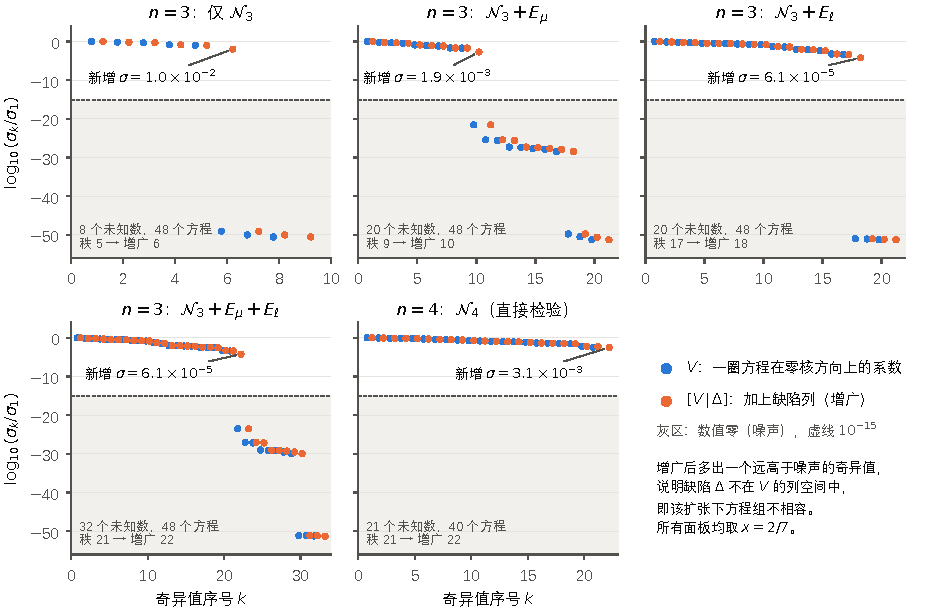
\includegraphics[width=\textwidth]{fig_spectra.pdf}
\caption{一圈方程系数矩阵 $V$ 与增广矩阵 $[V\,|\,\Delta]$ 的奇异值谱（归一化到 $\sigma_1$）。蓝、橙点左右错开画出。增广后在噪声线（虚线 $10^{-15}$）之上多出一个奇异值，即缺陷不在列空间中。前四幅为 $n=3$ 的扩张检验，右下为 $n=4$ 的直接检验。}
\label{fig:spectra}
\end{figure}

\FloatBarrier
%=====================================================================
\section{结论状态总表}
%=====================================================================
\begin{center}\small
\begin{tabularx}{\textwidth}{@{}>{\raggedright\arraybackslash}Xl@{}}
\toprule
结论 & 状态 \\ \midrule
$n=3$ 树级代表 \eqref{eq:Ktree} 对全部 helicity 成立 & \Proved \\
$\dim\N_3=8$ 及 8 条显式关系 & \Proved \\
$\Mone_{++}=0$；single-minus 闭式 \eqref{eq:M1sm} & \Exact \\
缺陷 $\Delta_3$（给定一圈输入）；$\Delta_3^{++}$ 闭式 \eqref{eq:Dap} & \Exact \\
定理~\ref{thm:n3}：$n=3$ 整个允许类不可能 & \CAProved \\
定理~\ref{thm:alln}：所有 $n\ge3$ 不可能 & \CAProved \\
$n=4$ 直接秩检验不相容 & \Numer \\
插入表示 \eqref{eq:insertion} & \Numer \\
四维 cut 全为零、缺陷来自 $\mu^2$ 项 & \Numer \\
$E_\mu$、$E_\ell$ 及合并扩张均失败 & \Numer \\
\bottomrule
\end{tabularx}
\end{center}

%=====================================================================
\section{尚未闭合的步骤与下一步检验}
%=====================================================================
\begin{enumerate}
\item single-minus EYM 闭式 \eqref{eq:M1sm} 由精确重构得到，尚无解析推导；证书只依赖 $p_0$ 处的三个值（已独立精确重构）。升级路径：从 \eqref{eq:insertion} 直接做 $\mu$ 积分。\hfill\Conj
\item 插入表示 \eqref{eq:insertion} 的推导依赖两点：$D$ 维 cut 决定有理项（Bern–Morgan），以及命题~\ref{prop:ins}。后者只在 $k\le4$ 个胶子、随机有理点上精确验证，未给出一般证明。\hfill\Conj
\item $n=4$ 直接检验尚为数值结论；用精确算术（90 位 + 有理重构）重做，可把它升级为证书。
\item 找出 $E_\ell$ 类扩张还缺少的最小结构（例如 $a\,|\,$圈线$\,|\,b$ 的非平面构型，或双迹部分振幅），并在 $n=3$ 检验，可作为可证伪的下一步。
\end{enumerate}

\appendix
%=====================================================================
\section{证书点数据}\label{app:data}
%=====================================================================
证书点 $p_0$（顺序为 $1,2,3,P$）：
\[
\lambda=(4,-3),\,(3,-2),\,(4,-4),\,(1,2);\qquad
\tilde\lambda=(-1,-3),\,(2,2),\,(-\tfrac{5}{12},\tfrac{17}{12}),\,(-\tfrac13,\tfrac13).
\]
\begin{table}[h]
\centering\small
\caption{$p_0$ 处的一圈 EYM 值与代表核的缺陷（本约定）。}\label{tab:p0}
\begin{tabular}{@{}lll@{}}
\toprule
扇区 & $\Mone$ & $\Delta_3(x)$ \\ \midrule
all-plus & $0$ & $(8x^2+6x-3)/5346$ \\
minus 在 1 & $-73/248832$ & $(18x^2-242x+169)/248832$ \\
minus 在 2 & $-65/235224$ & $-7(2x-1)/29403$ \\
minus 在 3 & $-185/13068$ & $(242x^2-466x+57)/13068$ \\
\bottomrule
\end{tabular}
\end{table}
证书：$y=(1,-\tfrac{11}{8},-\tfrac{11}{768})$ 作用在后三行，$y\cdot V\equiv0$，$y\cdot\Delta=-(2x^2-2x-3)/10368$。

\FloatBarrier
%=====================================================================
\section{复现文件}\label{app:files}
%=====================================================================
全部位于 \texttt{q1/}：
\begin{center}\small
\begin{tabularx}{\textwidth}{@{}lX@{}}
\toprule
文件 & 内容 \\ \midrule
\texttt{trees.py} & 由作用量导出的色序 Feynman 规则与 Berends–Giele（胶子、伴随复标量、$O(\kappa)$ 引力子） \\
\texttt{kin.py}, \texttt{exactpt.py}, \texttt{symx.py} & 有理旋量运动学、$\Q(x)$ 域、有理重构 \\
\texttt{collinear.py}, \texttt{colK.py} & $\Pi_n$、$\Cx$ 构型、树级核方程 \\
\texttt{loop.py}, \texttt{opp.py} & $D$ 维幺正性与 OPP（调和基、$\mu^{2r}$ 积分、退化 cut、插入表示） \\
\texttt{ym\_formulas.py}, \texttt{eym\_formulas.py} & YM 一圈解析式（本约定）、EYM $n=3$ 闭式 \\
\texttt{tree\_n3K.py}, \texttt{symbolic\_tree\_n3.py} & $n=3$ 树级核空间与符号证明 \\
\texttt{oneloop\_n3.py}, \texttt{cert\_n3*.py} & $n=3$ 一圈缺陷与不可解性证书 \\
\texttt{soft\_gluon.py}, \texttt{test\_soft*.py} & 软胶子与软引力子核验 \\
\texttt{ext\_test.py}, \texttt{ext\_analyze.py} & 扩张 $E_\mu$、$E_\ell$ 检验 \\
\texttt{n4\_direct.py}, \texttt{n4\_analyze.py} & $n=4$ 直接检验 \\
\texttt{paper/fig\_spectra.py} & 图~\ref{fig:spectra}（数据：\texttt{spectra\_n3.json}, \texttt{spectra\_n4.json}） \\
\bottomrule
\end{tabularx}
\end{center}

\end{document}
